\scanpage{82}
\margin{81}
or equivalently, by the $g^\alpha_{x,y}$ \inserted{$\in\widehat\Pi_\alpha$}, where $\alpha\in A$, $x,y\in I_\alpha$ (cf above). This recalled,
\margin{\figure{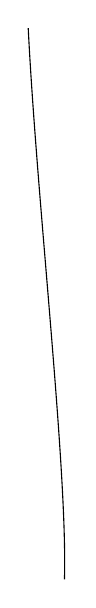
\begin{tikzpicture}\draw (0,0)..controls(.04,1.4)and(-.35,4.8)..(-.46,7);\end{tikzpicture}}}
one can hope to give explicit ``formulas'', \uline{depending of course on the precise arithmetic properties of the particular point} $x$, and \uline{characteristic of} $x$ (in the Mordell-Weil-Néron situation), which give $f_l(u)$ \uline{in terms} of the preceding parameters fixing $u$. That is fascinating work in prospect, which I have practically not begun yet for the moment!

To tell the truth, the proof via Mordell-Weil of the uniqueness of an $x$ \inserted{$\in X_K$} which corresponds to a given class in $H^1(\Gamma,\widehat\Pi_1(x_0))$, shows that one has uniqueness even if one \deleted{\unsure{gives of it}} \inserted{\unsure{knows|knows}} only the element corresponding to \deleted{\unsure{a}}
\[
\tag{34}(f_{x_0,x})_{\mathrm{ab}}\in H^1(\Gamma,\widehat\Pi_1(X,x_0)_{\mathrm{ab}}),
\]
and one can already try to determine, by ``explicit formulas'', the $(f_l)_{\mathrm{ab}}$ corresponding to paths $x_0\longrightarrow x$. One is reduced to looking at the same question by replacing $X$ by an abelian variety or extension thereof,

\margin{(This is a particular question, which \unsure{much more interesting|most interesting} \illegible{?} \unsure{a problem|a formula} \unsure{variable|valid} \unsure{in} $X$ \unsure{over} $\unsure{\mathbb Q}$ \illegible{?}\unsure{.)}}
